


% ANUfinalexam.tex (Version 2.0)
% ===============================================================================
% Australian National University Final Exam LaTeX template.
% 2004; 2009, Timothy Kam, ANU School of Economics
% Licence type: Free as defined in the GNU General Public Licence: http://www.gnu.org/licenses/gpl.html

\documentclass[a4paper,12pt,fleqn]{article}
\setlength{\parindent}{0em}
\usepackage{amsmath}
\usepackage{fancyhdr}
\usepackage{siunitx}
\usepackage{enumitem}
\usepackage{amsmath}
\usepackage{graphicx}
\usepackage{tikz}
\usepackage{import}
\usepackage{comment}

% Unit definitions %%%%%%%%%%%%%%%%%%%%%%%%%%%%%%%%%%

\DeclareSIUnit\kilowatthour{kWh}
\DeclareSIUnit\kilowattpeak{kW_P}
\DeclareSIUnit\kVA{kVA}
\DeclareSIUnit\kVAR{kVAR}
\DeclareSIUnit\year{y}
\DeclareSIUnit\north{N}
\DeclareSIUnit\south{S}
\DeclareSIUnit\second{s}
\DeclareSIUnit\mmhg{mmHg}


% Insert your course information here %%%%%%%%%%%%%%%%%%%%%%%%%%%%%%%%%%

\newcommand{\institution}{CORNWALL COLLEGE}
\newcommand{\titlehd}{BSc Environmental Resource Management}
\newcommand{\examtype}{Exam}
\newcommand{\examdate}{Academic Year 2015-2016}
\newcommand{\examcode}{ERM304}
\newcommand{\examtitle}{Research Methods}
\newcommand{\readtime}{15 Minutes}
\newcommand{\writetime}{Three Hours}
\newcommand{\materials}{Non-programmable Calculators}
\newcommand{\middlewords}{Exam continues on next page}
\newcommand{\lastwords}{End of Exam}

%%%%%%%%%%%%%%%%%%%%%%%%%%%%%%%%%%%%%%%%%%%%%%%%%%%%

%\setcounter{MaxMatrixCols}{10}
\newtheorem{theorem}{Theorem}
\newtheorem{acknowledgement}[theorem]{Acknowledgement}
\newtheorem{algorithm}[theorem]{Algorithm}
\newtheorem{axiom}[theorem]{Axiom}
\newtheorem{case}[theorem]{Case}
\newtheorem{claim}[theorem]{Claim}
\newtheorem{conclusion}[theorem]{Conclusion}
\newtheorem{condition}[theorem]{Condition}
\newtheorem{conjecture}[theorem]{Conjecture}
\newtheorem{corollary}[theorem]{Corollary}
\newtheorem{criterion}[theorem]{Criterion}
\newtheorem{definition}[theorem]{Definition}
\newtheorem{example}[theorem]{Example}
\newtheorem{exercise}[theorem]{Exercise}
\newtheorem{lemma}[theorem]{Lemma}
\newtheorem{notation}[theorem]{Notation}
\newtheorem{problem}[theorem]{Problem}
\newtheorem{proposition}[theorem]{Proposition}
\newtheorem{remark}[theorem]{Remark}
\newtheorem{solution}[theorem]{Solution}
\newtheorem{summary}[theorem]{Summary}
\newenvironment{proof}[1][Proof]{\noindent\textbf{#1.} }{\ \rule{0.5em}{0.5em}}

% ANU Exams Office mandated margins and footer style
\setlength{\topmargin}{0cm}
\setlength{\textheight}{9.25in}
\setlength{\oddsidemargin}{0.0in}
\setlength{\evensidemargin}{0.0in}
\setlength{\textwidth}{16cm}
\pagestyle{fancy}
\lhead{} 
\chead{} 
\rhead{} 
\lfoot{} 
\cfoot{\footnotesize{Page \thepage \ of \pageref{finalpage} -- \titlehd \ (\examcode)}} 
\rfoot{} 

% DEPRECATED: ANU Exams Office mandated margins and footer style
%\setlength{\topmargin}{0cm}
%\setlength{\textheight}{9.25in}
%\setlength{\oddsidemargin}{0.0in}
%\setlength{\evensidemargin}{0.0in}
%\setlength{\textwidth}{16cm}
%\pagestyle{fancy}
%\lhead{} %left of the header
%\chead{} %center of the header
%\rhead{} %right of the header
%\lfoot{} %left of the footer
%\cfoot{} %center of the footer
%\rfoot{Page \ \thepage \ of \ \pageref{finalpage} \\
%       \texttt{\examcode}} %Print the page number in the right footer

\renewcommand{\headrulewidth}{0pt} %Do not print a rule below the header
\renewcommand{\footrulewidth}{0pt}


\begin{document}

% Title page

\begin{center}
%\vspace{5cm}
\large\textbf{\institution}
\end{center}
\vspace{1cm}

\begin{center}
\textit{ \examtype -- \examdate}
\end{center}
\vspace{1cm}

\begin{center}
\large\textbf{\titlehd}
\end{center}

\begin{center}
\large\textbf{\examcode}
\end{center}
\begin{center}
\large\textbf{\examtitle}
\end{center}
\vspace{4cm}
\vspace{4cm}

\begin{center}
%\textit{Reading Time: \readtime}
\end{center}
\begin{center}
\textit{Time Allowed:  \writetime}
\end{center}
\begin{center}
\textit{Permitted Materials: \materials}
\end{center}

% End title page
\newpage
\large{\textbf{Instructions}}\newline\newline
\large{You must answer TWO out of Questions 1, 2 and 3.}\newline\newline
\large{You MUST answer Question 4.}\newline\newline
\large{All Questions carry equal weight.}\newline\newline

\newpage


\bigskip

\textbf{\large{Answer any TWO of Questions 1, 2, and 3}}\newline

%\vspace{0.5cm}

\textbf{Question 1}\newline

With reference to relevant examples, identify and illustrate the main features of a convincing scientific argument.

\vspace{1cm}

\textbf{Question 2}\newline

Describe a current or recent research programme related to environmental science and comment on the extent to which the ideas of Kuhn, Popper, Lakatos or Feyerabend provide an adequate account of the conduct of individuals involved and the development of the programme. 

\vspace{1cm}

\textbf{Question 3}\newline

With reference to examples, assess the role, impact and limitations of the process of peer review within scientific practice.

\vspace{1cm}

\textbf{\large{You MUST answer Question 4}}\newline

\textbf{Question 4}\newline


	A healthy systolic blood pressure in adults is about 120 mmHg, with a standard deviation among the adult population of about 12 mmHg. \newline
	
	A pharmaceutical company has devised a drug which it hopes will reduce blood pressure by \SI{3}{\mmhg}. This is deemed the minimum reduction that would merit the risks of taking the drug. A research group is asked to test whether this reduction in pressure actually happens and plan to report that the drug does reduce blood pressure if they find a reduction for which the p-value is 0.05 or less. In a first attempt, the investigators make measurements of blood pressure on a treatment group of 100 randomly chosen individuals who have had the drug, and on a control group of another 100 randomly chosen individuals who have taken a placebo drug instead.  The mean blood pressures for each group are then calculated.\newline
	
	
	The pooled standard error of the difference  $\bar{x}_\text{trmt}-\bar{x}_\text{ctrl}$ between the mean pressures of the two samples is 1.7 mmHg.

\begin{enumerate}[label=\alph*)]
\item	
	\begin{enumerate}[label=\roman*)]
	\item In this investigation, double blinding was used. What is this and why is it used here?
	\item What is the standard error of the mean blood pressures $\bar{x}_\text{trmt}$ and $\bar{x}_\text{ctrl}$ of each group?
	\item Write down suitable hypotheses for a two sided hypothesis test in this context.
	\item Under the null hypothesis, what would be the mean difference between the mean values of blood pressure from each sample $\bar{x}_\text{trmt}-\bar{x}_\text{ctrl}$
	\end{enumerate}
	
	\item Study Figure 1 below which shows probability distributions of measured differences of the means under the null hypothesis and under the alternate hypothesis in which there is a reduction in blood pressure of \SI{3}{\mmhg}. The dashed vertical lines indicate the limits of the regions of rejection of the null hypothesis, at the 5\% significance level. 
	
	\begin{enumerate}[label=\roman*)]
	\item Explain why the dashed lines are positioned at about $ \pm\SI{3.4}{\mmhg}$.
	\item Comment on whether this investigation has been well designed for its purpose of detecting an an effect of at least \SI{-3}{mmhg}
	\item  Supposing that a real effect does \emph{not} exist, give with justification  an example of a measured value for the mean pressure difference that would give rise to a Type 1 error
	\item  Supposing that a real effect of \SI{-3}{\mmhg} \emph{does} exist, give with justification  an example of a measured value for the mean pressure difference that would give rise to a Type 2 error

	\end{enumerate}
	\begin{figure}[h]
	\centering
	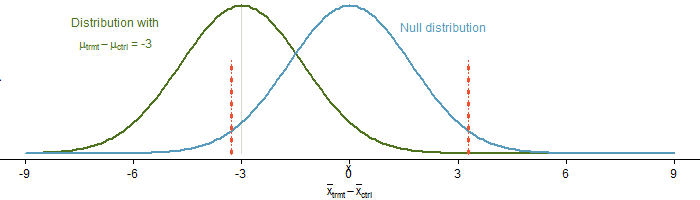
\includegraphics[width=0.85\textwidth]{power_null_C_0_1_7_with_alt_at_3.png}
	\caption{Probability distribuitions for the alternate hypothesis (left) and null hypothesis (right). The dashed lines indicate the limits of the regions of rejection of the null hypothesis at the 5\% significance level.}
	\label{figure:q3b}
	\end{figure}
	
	\item A Research Council requires that any experimental investigation it funds should be designed in such a way as to ensure 80\% power. 
	\begin{enumerate}[label=\roman*)]
	\item Explain the meaning of the term 'power' in this context.
	\item  Estimate the approximate power of the investigation and give your reasoning.
	\item What could the investigators do to improve the power of their investigation?
	\end{enumerate}
	
	
	
%	\item Ionnadis (2005) made the startling claim in a peer-reviewed article that "most published research findings are false". 
%	
%	We can explore this statement using the following relation. 
%	
%	\begin{align*}
%	\mathrm{Posterior\ odds} &= \mathrm{Bayes\ Factor}\times\mathrm{Prior\ odds}\\
%	&=\left(\dfrac{\mathrm{power}}{\mathrm{1-specificity}}\right)\times\mathrm{Prior\ odds}
%	\end{align*}

	Suppose the investigators find that the mean blood pressure of the treatment group is \SI{3.7}{mmhg} lower than that of the control group. The p-value for this result is 0.015 and hence the investigators claim to have evidence sufficient to reject the null hypothesis.
	\begin{enumerate}[label=\roman*)]
	\item Explain in English what this p-value means.
	\item A peer-reviewer states, correctly, that investigators cannot infer with 98.5\% probability that the null hypothesis must be false. Explain why the peer-reviewer is correct.
	\item Explain from a Bayesian perspective what additional information would be needed in order to assess the odds for the truth or otherwise of the null hypothesis.
	\end{enumerate}	
%	Let us take the example of a disease, for which the prevalence is 0.1, and for which we have a test. The sensitivity and specificity of this test are both 0.9. 
%	
%	\begin{enumerate}[label=\roman*)]
%	\item What is meant by the term "odds"
%	\item Calculate the posterior odds in this case.
%	\item Given a positive test on someone, is it more likely than not that the person actually has the disease.
%	\item Suggest  how the circumstances under which Ioannidis's statement might be correct could be avoided.
%	
%	\end{enumerate}
\end{enumerate}

\begin{center}
\vspace{3cm}
--------- \textit{\lastwords} ---------
\end{center}


\label{finalpage}

%\begin{comment}

\newpage
\textbf{\large{Solution}}\newline\newline
\textbf{Solution to Question 1}\newline

A good answer will include many of the following points:
\begin{itemize}
\item Rationale,context provided
\item Relevant and credible literature cited
\item Scope, aims, objectives presented
\item Exclusions described, with rationale
\item Terms, concepts defined
\item Relevance of terms, concepts explained
\item Methodology cited, used clearly presented and transparent
\item Methodology appropriate
\item Evidence presented
\item Sufficient evidence
\item Appropriate comment on the evidence
\item Relevance of evidence explained
\item Appropriate analysis of evidence
\item Comment on limitations, omissions, inconsistencies
\item Conclusions justified by evidence
\item Discussion of scope of conclusions
\item Uncertainties, errors etc discussed and quantified where possible
\item Impact of methodology on results, reliability of conclusions explained
\item Next steps outlined
\item Language, level of detail etc, appropriate for audience
\item Clear, structured presentation
\end{itemize}

\textbf{Solution to Question 2}\newline

Good answers to provide evidence of understanding of ideas of K, P, L and F and of their relevance to chosen research programme. Answers might include the following:

\begin{enumerate}[label=\alph*)]
\item Kuhn
\begin{enumerate}[label=\roman*)]
\item Paradigm explained
\item Response of actors to anomalies
\item Consequence of profusion of anomalies
\item Daily reality of practising scientists
\item Examples
\end{enumerate}

\item Popper
\begin{enumerate}[label=\roman*)]
\item Idea of falsifiability explanatory power as filter for science / non science. Confirmations rather than proof
\item Identifiable progress within the field as a consequence of falsification of hypotheses.
\item  Lack of progress a consequence of untestable ideas? 
\item Examples
\end{enumerate}

\item Lakatos
\begin{enumerate}[label=\roman*)]
\item Consistency, commensurability the key issue
\item Limitations of simplistic falsifiability
\item Complex issues, lack of smoking gun experiments
\item Actual response of actors to experimental results
\item Research programmes rather than individual theories
\item Examples
\end{enumerate}

\item Feyerabend
\begin{enumerate}[label=\roman*)]
\item Do actors agree on an objective reality and on primacy of evidence?
\item Is there a diversity of approaches (eg alternative/mainstream)?
\item Strengths / dangers of mulitiplicity of approaches discussed.
\item Professionalisation/centralisation of science – dangers/strengths
\item Relativist attacks on science
\item Perceptions of balance
\item Examples
\end{enumerate}
\end{enumerate}


\textbf{Solution to Question 3}\newline

Credit
\begin{itemize}
\item Journals / editors/referees/iterative process between submission and decision
\item Criteria for decision : appropriate for journal; meets house rules of journal; context; methodology, analysis, conclusions justified by analysis; priority
\item Role of anonymity : advantages, disadvantages
\item Function as filter; quality assurance of published scientific record; role within career and funding decisions
\item Limitations : inherently conservative? Makes science too slow to respond rapidly when required?
\item Safeguards : against unfair stealing of ideas (submission dates, multiple referees)
\item Examples : distinction between peer review journals and the rest, inc grey literature; consequences of reliance upon grey literature alone
\item Awareness of different models of peer review currently in use, and a balanced discussion of their relative pros and cons.
\item Discussion of role of peer review in light of emergence of pre-print sites
\end{itemize}

\textbf{Solution to Question 4}\newline
\begin{enumerate}[label=\alph*)]
\item
\begin{enumerate}[label=\roman*)]
	\item To avoid bias on the part of the subjects or the researchers.
	\item $\text{SE}=\dfrac{\text{SD}}{\sqrt{N}}=\dfrac{12}{\sqrt{100}}=1.2$
	\item Null Hypothesis: the drug has no effect on blood pressure so that $\mu_\text{trmt}=\mu_\text{ctrl}$; Alternate: The drug changes blood pressure so that $\mu_\text{trmt}\neq\mu_\text{ctrl}$
	\item 0
\end{enumerate}
\item 
\begin{enumerate}[label=\roman*)]
\item They are 2 (1.96) SE's away from the null mean, and so there is a 5\% probability that the data will lie beyond the, if the null mean is true.
\item Not really The effect to be detected has size -3 mmHg, but if this were the detected difference made by the drug, the combination of effect size and significance level mean that the null would not be rejected.
\item False positive. An effect greater than $ \pm\SI{3.4}{\mmhg}$ eg - 3.7 mmHg
\item False negative.  An effect less than $ \SI{3.4}{\mmhg}$ eg -2.7 mmHg
\end{enumerate}
\item
\begin{enumerate}[label=\roman*)]
\item The likelihood that a real effect wil lbe detected.
\item Accept $\approx 45$\%
\item Cannot change effect size or SD of population, so can increase sample size to reduce SE.
\end{enumerate}
\item
\begin{enumerate}[label=\roman*)]
\item The probability that data as or more extreme than that actually measured would have been obtained \emph{given} that the null hypothesis is true.
\item If measuring an effect of greater than -3 mmHg, at 5\% significance level is denoted "+", and if the null hypothesis is denoted $H_0$, then the p-value is $P(+|H_0)$ = 0.015. The probability that the null hypothesis is false, and thus that the alternative hypothesis $H_A$ is true, given the positive result, iS $P(H_A|+)=1-P(H_0|+)$, but it is not generally the case that $P(H_0|+)=P(+|H_0)$
\item Prior odds required - assessment of odds that effect exists, prior to doing doing the measurements.
\end{enumerate}
\end{enumerate}



%\end{comment}

\end{document}

